\hyphenation{ma-te-rials}
%%%%%%%%%%%%%%%%%%%%% Introduction %%%%%%%%%%%%%%%%%
\chapter{Introduction}
\label{ch:intro}

When one of the brightest physicists that has ever lived on Earth, Richard Feynman, was asked to summarise in one single phrase everything that we know about the world around us, he said, "all things are made of atoms" \cite{Feynman_atoms}. Feynman himself was the father of the quantum electrodynamics and definitely knew how to answer that question. In this simple response to general public he decided not go into quantum mechanics principles and rather illustrated at the highly abstract level that everything is made of smaller particles. For example, nowadays we know that atoms have nuclei and electrons on the electron shells, "orbiting" around the nucleus. The nucleus is positively charged proportionally to the number of protons it contains. To provide the stability of the nuclei of the heavy atoms our world also needs neutrons, which have no electric charge. Also neutrons decay, a free neutron decays weakly in about 15 minutes, while the proton is stable, as far as we know from the experiments, and only in some Beyond the Standard Model (BSM) theories it is hypothesised that the proton lifetime is finite. However, the estimate of the proton lifetime is a value that is larger than the age of our Universe and is at least $10^{30}$ years \cite{DIMOPOULOS1982133}. Going further to an even smaller scale, we can say that protons and neutrons are not elementary, instead they are composed of point-like constituents that are called quarks (see Figure \ref{atom_structure}). 

\begin{figure}[H]
  \centering
    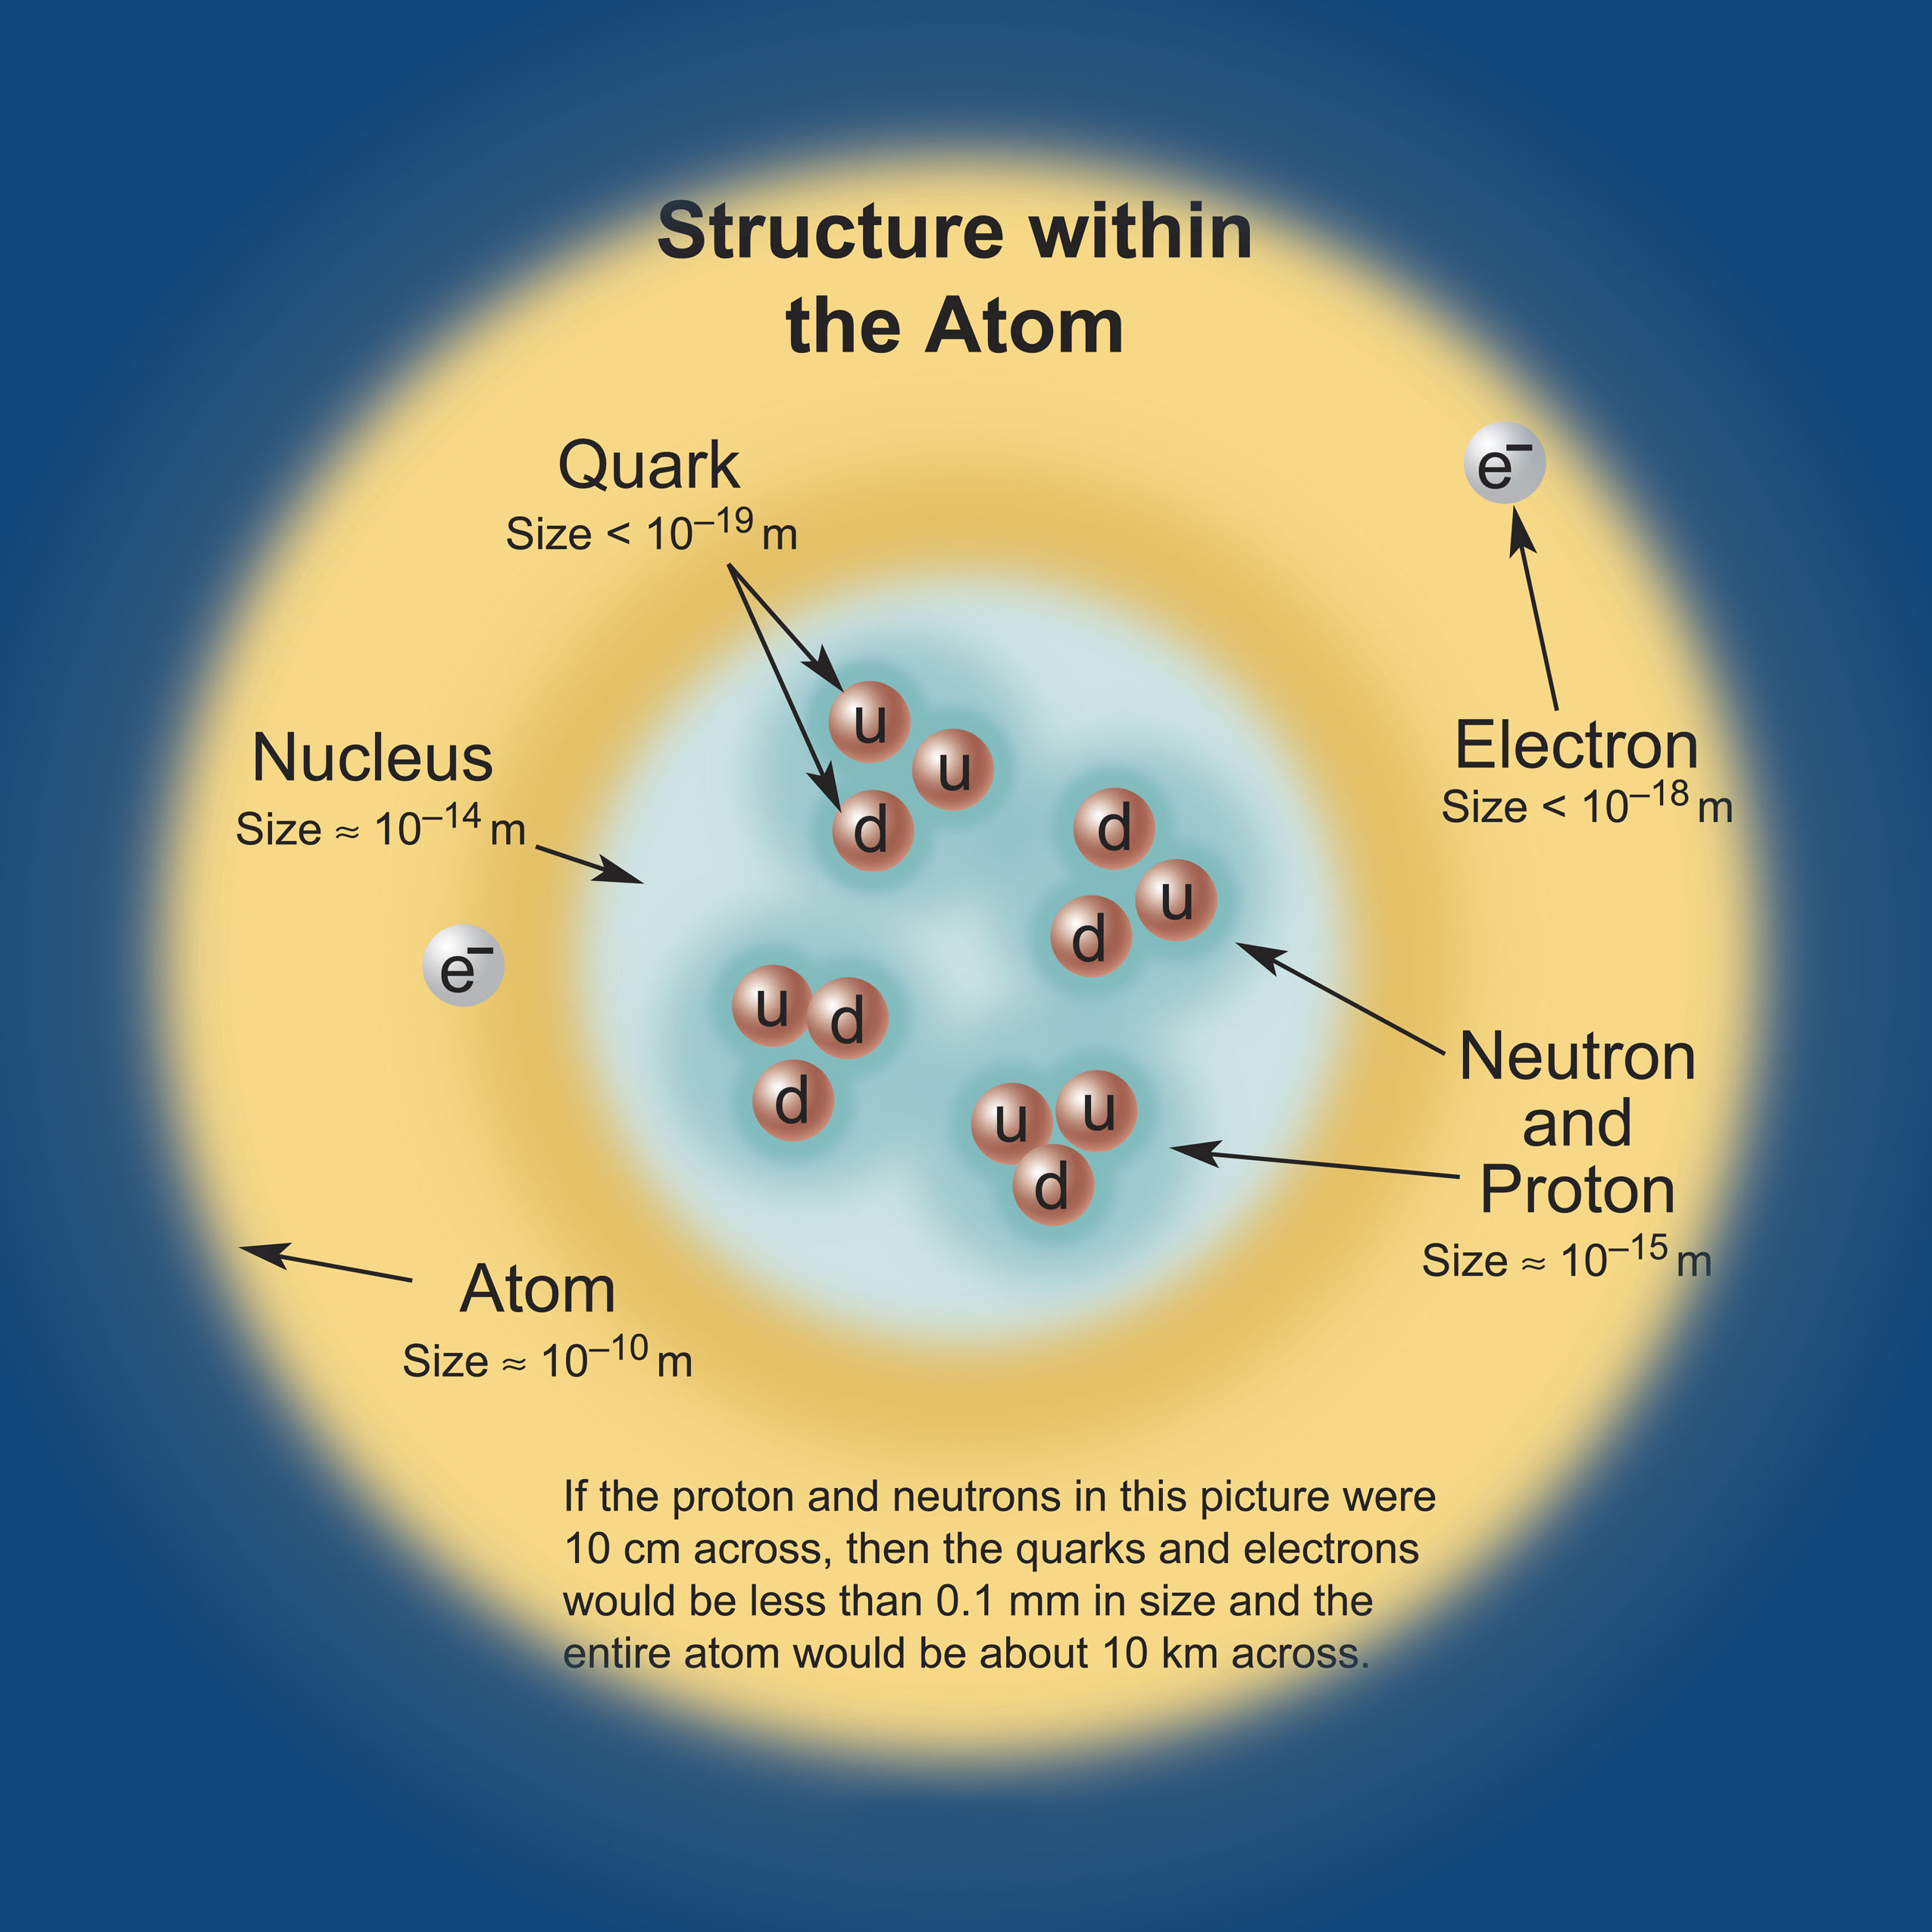
\includegraphics[width=0.70\textwidth]{atom_structure}
    \caption{The structure of the atom. Approximate scale values are indicated.}
    \label{atom_structure}
\end{figure}

Quarks were proposed by Gell-Mann and also by Zweig to explain why Eightfold Way works  \cite{griffiths_hep}. Quarks come come in three families, or generations, and are arranged into doublets. Each doublet has an "up" quark with the charge $-1/3$ and a "down" quark with the charge $+2/3$. For antiquarks signs are reversed of course. These peculiar detail about their charge number being fractional was so much revolutionary at that time, that Gell-Mann decided not to publish his article in highly prestigious journal, but expecting a rejection, decided to go with the second tier one \cite{griffiths_hep}. In addition to a charge number, quarks also have a "flavor" number assigned to them. For instance, a charm quark has $+1$ unit of "charmness", while a strange quark has $-1$ unit of "strangeness". All the other quark flavor fields are zero for them. And this pattern is applied to all the other four quarks to fill the corresponding "quarkness" numbers. Another detail worth mentioning about quarks is that the mass of quarks increases from the first to the third family. No explanation exists in the Standard Model (SM), masses are the parameters in this theory, but perhaps the so-called "The Theory of Everything", which is to be written (had been a lifelong journey of another genius, Einstein \cite{aps_einstein}), will be able to explain such phenomenon. But it is not the whole description of quark properties. Another important characteristics of quarks has been revealed at the $e^+e^-$ colliders when analysers compared final cross sections in hadronic and muonic states. The theory was off by a factor of three. And this was the motivation to introduce three quark colors: green, blue, and red. 


Since it was mentioned that the atoms contain electrons, it is a good time to talk about leptons. An electron, the first lepton to be officially observed in the experiment, was discovered by Thompson \cite{Davis:1989898} in 1897 when he was studying the properties of a cathode ray. That year is of a great importance, since it gave birth to an era of a modern particle physics. Almost 40 years later, in 1936, a muon was discovered \cite{Piccioni1996} in an experiment of Carl Anderson and Seth Neddermeyer who studied cosmic radiation. A muon is almost a copy of an electron, but is 207 times heavier. There is a story that Feynman was able to derive the mass of the muon starting with the mass of an electron, but the world has never seen that calculation been published \cite{Bender}. 

Analogously to quark families, leptons are also arranged in generations. Each generation is a doublet that consists of a charged lepton (electron, muon or tau) with the charge $-1$ and a neutral lepton (corresponding electron, muon, or a tau neutrino). An electron and a muon neutrinos have been discovered in 1956 and 1962 respectively. The existence of the first one was deduced from the violation of the conservation of energy in a beta decay, while the muon neutrino \cite{PhysRevLett.9.36} was discovered by Schwartz, Lederman, and Steinberger during a several months long experiment with the pion beam, which was an experiment that counted events that pass the steel wall and arrive to the aluminum spark chamber. They accumulated 51 events of interest. Those events could not be due to electron neutrinos, since they will interact with the aluminum. The presence of muons in each event was a clear indication that those neutrinos were of a different kind, they were muon neutrinos. After some time, a tau lepton and a tau neutrino were discovered in 1975 and 2000 correspondingly \cite{PhysRevLett.35.1489, Kodama:2000mp}. With that, the SM pattern for leptons was completed and a long-awaited tau neutrino, which was theoretically speculated to exist, was finally observed experimentally. And likewise to families of quarks, lepton masses grow with the generation, where the top quark from the third generation is the heaviest particle in the whole SM. To help identify leptons of different families the lepton numbers have been reserved: 1 unit of electron number to an electron and an electron neutrino, 1 unit of muon number to a muon and an muon neutrino, and 1 unit of tau number to a tau and a tau neutrino. And a final remark on neutrinos, in the SM they are massless, however, it has been shown that they have a non-zero mass \cite{Bilenky:2014ema}. This fact is one of the main motivations for theorists to look for extensions of the SM. 

\begin{figure}[H]
  \centering
    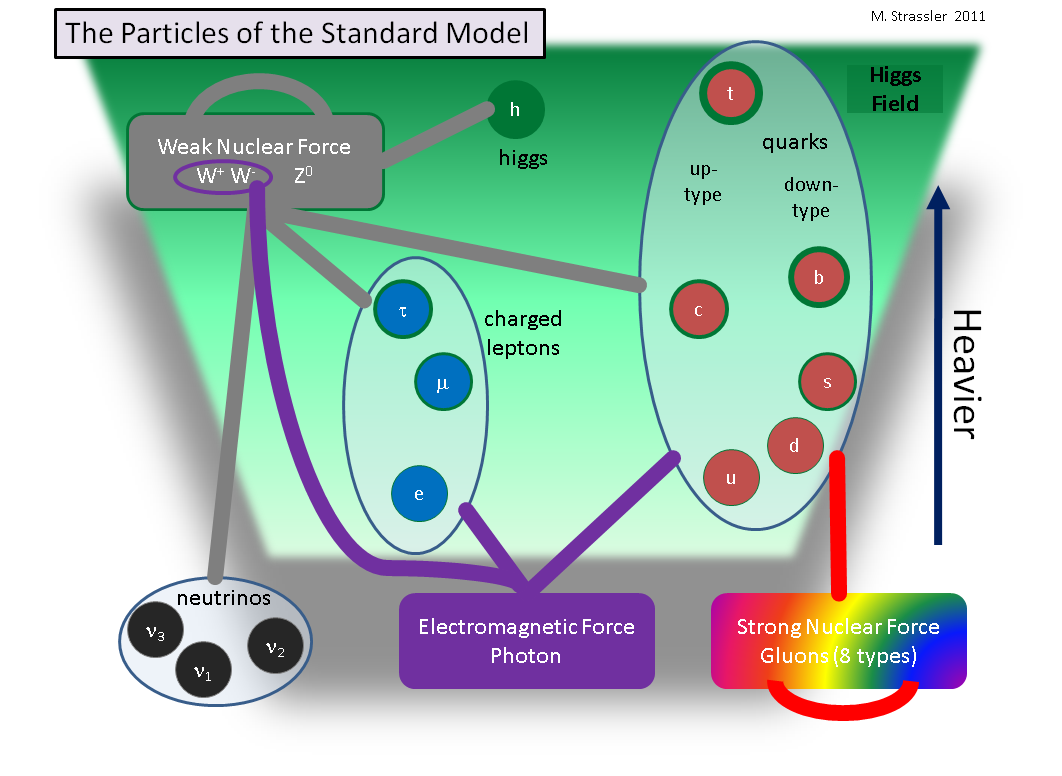
\includegraphics[width=0.90\textwidth]{sm_interactions2}
    \caption{SM particles and force carriers \cite{strassler}. Self-interactions are also shown. The strength of the coupling to the Higgs boson increases from the bottom to the top, which is illustrated by the shades of the green color (the Higgs field).  }
    \label{sm_interactions2}
\end{figure}

At the fundamental level the world is made of quarks and leptons. And there must be rules, at least we expect them to exist, which explain how quarks/leptons interact. These rules are referred to as fundamental forces of nature. As of now, there exist four: gravitational, weak, electromagnetic, and strong forces. The first one governs the Universe at the macroscopic level: planets, solar systems, etc. The first theory of gravity was formulated by Newton \cite{Chandrasekhar:1187874} and then further developed by Einstein. A good historical perspective is available at \cite{Gutfreund:1980674}. Worth noting that the gravitational force is not included in the SM. Attempts are ongoing to expand the SM, e.g., adding the graviton as a mediator, but no real success so far to have a renormalizable theory that would combine both SM and gravity \cite{butterworth2014smashing}. 

Throughout this thesis the so-called natural system of units is adopted, in which $\hbar = c = 1$. This simplifies how many equations look and also makes a fine-structure constant $\alpha \approx 1/137$ dimensionless.
Following this convention \cite{Cottingham:1026625}, masses, momentum, and energies are measured in electronvolts (eV), with GeV ($10^9 ~eV$) and TeV ($10^{12}~eV$) being the most popular units in a modern high-energy physics due to energy regimes involved.

We will classify all four forces \cite{wolfram} in terms of the relative strength, the range that they can cover, the spin of the mediator, and whether the force's nature is attractive, repulsive, or both. This should be taken with the grain of salt though, since this is quite ambiguous categorisation, but it has a deep pedagogical meaning because helps to illustrate in which regime each of the forces is dominant. And this is the main physics objective - to know which effects are the dominant, which are sub-dominant, and which can be neglected so that correct approximations could be made and it would become possible to do calculations for problems where closed-form solutions do not exits, which is almost all the phenomena around us \cite{Bender}. Gravity is the weakest force, the only reason why the motion of planets and galaxies is governed by gravity is because those are gigantic objects and this enormous number of involved particles pushes gravity effects to be the dominant ones at the macroscopic scale. If the strength of the strongest force, which is the strong force, is set to 1, then the strength of the gravity will be about $10^{-41}$. It is contemplated that the gravity mediator (the graviton), if exists, would have a charge of zero, zero mass, spin 2, and should be a stable particle. The gravitational force is of the infinite range and its nature is purely attractive, while all other three forces can exhibit both an attractive and a repulsive behaviour. Einstein's general relativity theory is the only proven working theory of gravity as of now, though not a quantum theory, and sometimes is called "geometrodynamics". 

The next force we are going to discuss is the weak force. It is mediated by a W (charge +1/-1) boson or a neutral Z boson, thus giving name to charged and neutral weak interactions correspondingly. All SM fermions experience the weak force, both quarks and leptons. For leptons, it worth mentioning here that neutral leptons have no charge, thus will not participate in the electromagnetic interactions, and all leptons have no color charge, so they feel no strong force \cite{griffiths_hep}. The relative strength would be  $10^{-16}$ and the range of applicability is $10^{-3}$ fm. All three bosons have spin 1 and are quite massive $m_{W} = 80. 385$ GeV and $m_{Z}=91.189$ GeV. Since Z boson is neutral, any interaction where the photon is a force carrier, can be also mediated by the Z boson, see Fig. \ref{SM_vertices}.

\begin{figure}[H]
  \centering
    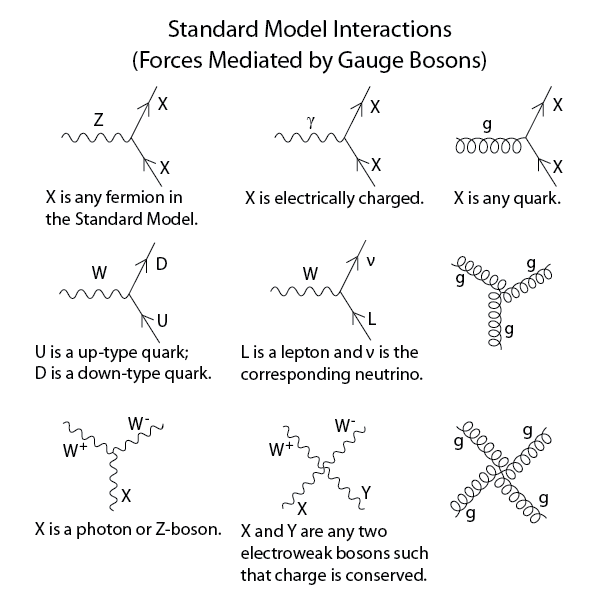
\includegraphics[width=0.80\textwidth]{Standard_Model_Feynman_Diagram_Vertices}
    \caption{All SM interaction and simple vertices. }
    \label{SM_vertices}
\end{figure}


For leptons charged weak interactions are interesting due to the fact that a primitive interaction vertex can be thought of as a point where a charged lepton is converted to a neutral lepton or vice versa. A good example is a muon decay, which is nothing but a conversion of the muon to a muon neutrino with the help of the W boson, which further decays to an electron and a corresponding electron antineutrino. What is also important is that lepton numbers are conserved and conversions happen only within the same family of leptons. 

Charged interactions do not conserve the flavor of quarks, e.g., members of doublets of the third and the second families can be converted into members of the lower family of quarks. This fact is reflected in the Cabibbo-Kobayashi-Maskawa (CKM) matrix, where diagonal elements are less than 1 and off-diagonal elements are non-zero, given by  

\begin{equation}
\small
\begin{pmatrix}
|V_{ud}| & |V_{us}| & |V_{ub}| \\
|V_{cd}| & |V_{cs}| & |V_{cb}| \\
|V_{td}| & |V_{ts}| & |V_{tb}|
\end{pmatrix} = \begin{pmatrix}
0.97427 \pm 0.00015 & 0.22534 \pm 0.00065 & 0.00351^{+0.00015}_{-0.00014} \\
0.22520 \pm 0.00065 & 0.97344 \pm 0.00016 & 0.0412^{+0.0011}_{-0.0005} \\
0.00867^{+0.00029}_{-0.00031} & 0.0404^{+0.0011}_{-0.0005} & 0.999146^{+0.000021}_{-0.000046}
\end{pmatrix}.
\label{eq:ckm}
\end{equation}






%\begin{figure}[h!]
%  \centering
%  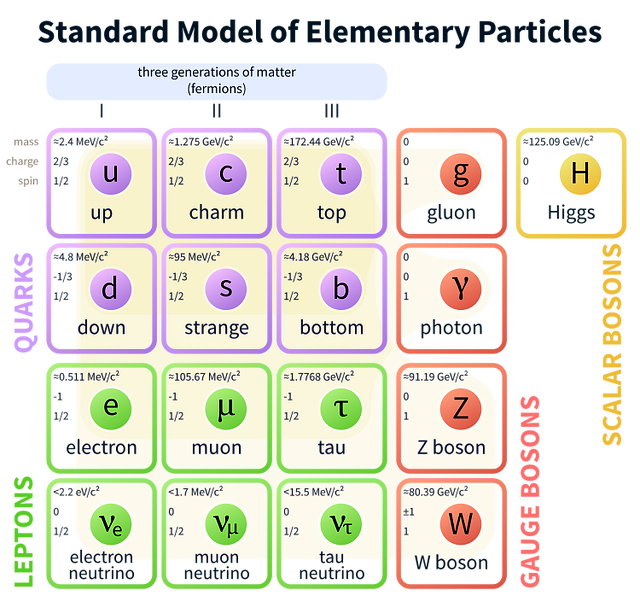
\includegraphics[scale=0.4]{sm}
%  \caption[Standard Model of particle physics.]{Schematic representation of the Standard Model of particle physics. The SM is a theoretical model intended to describe three of the four fundamental forces of the universe in terms of a set of particles and their interactions. \cite{smpicture}.}
%  \label{sm}
%\end{figure}
%


Moreover, W and Z bosons can couple to each other, so $WWZ, WWWW$, and $WWZZ$ vertices are possible in the SM. Finally, since W boson participates in charged interactions, it also couples to photons, so $\gamma WW$, $\gamma WWZ$, and $WW\gamma\gamma$ vertices are also allowed.

Now, we are moving to the electromagnetic (EM) force. This is the force that we experience in our everyday life. The reason the reader can sit in the chair and do not fall further down due to gravity, is that electrons of the reader's body repel electrons of the chair. Relative strength of the EM force is $10^{-3}$ and the range of applicability is infinite. A photon, as a mediator, has zero mass, spin 1, and the theory to describe its interaction with leptons and quarks is called quantum electrodynamics (QED), developed in 1940th and 1950th by Tomonaga, Schwinger, Feynman, Dyson \cite{qed_fathers}. Electric charge is conserved in EM interactions and no single photon-to-fermion vertex is possible, there are always two fermions that must be involved in such a way that their net electric charge is zero. 

Finally, talking about the strong force, this is the strongest known force, where the gluons are the carriers. There are nine types of gluons and each gluon carries one unit of color and one unit of anticolor. But technically, the ninth gluon is a color invariant, and would give rise to an infinite range of the strong force, which contradicts experiments. That is why physics literature states that in our world only eight gluons exist \cite{griffiths_hep, pdg}.

Gluons carry color charge and can couple to each other. For several high order processes in quantum chromodynamics (QCD), 3- and 4-gluon vertices have to be introduced to restore gauge invariance and no higher order vertices are required \cite{Mangano:454171}.
 
	
The whole SM picture will not be completed without the main particle yet missing until 2012th ... the Higgs boson! (Fig. \ref{sm_interactions2}) After the electroweak unification by Glashow, Salam, and Weinberg \cite{Glashow:1961tr}, it was still not clear what is the origin of the mass of fundamental particles. In 1964, Robert Brout and Fran�ois Englert\cite{PhysRevLett.13.321}, Peter Higgs\cite{PhysRevLett.13.508}, Gerald Guralnik, C. Richard Hagen, and Tom Kibble \cite{PhysRevLett.13.585} (BEHGHK authors), proposed the method by which the particles can acquire mass. 
This technique consists of three stages and we will discuss all three of them:

\begin{enumerate}
\item The Brout-Englert-Higgs (BEH) mechanism
%\begin{enumerate}
%\item Nested item 1
%\item Nested item 2
%\end{enumerate}
\item The BEH field
\item The Higgs boson.
%\ldots
\end{enumerate}

The BEH mechanism is simply a spontaneous symmetry breaking (SSB) mechanism, which is a mathematical trick consisting of rewriting the original scalar fields in the EW Lagrangian, rearranging equations, and requiring that the fields are real. What does this give? We started with a scalar complex field and a massless vector field and after SSB we got a single real scalar field (Higgs boson) and a massive vector field. In our physical world this gives mass to W and Z bosons. 

The BEH field exists everywhere and has been present almost since the Big Bang \cite{who_cares}. It is a property of our world. All the fundamental particles that interact with the BEH field acquire the mass. Those, who do not interact directly (at the tree level), have no mass and all their energy is in the form of the momentum, thus they can travel with the speed of light. The more the particle interacts with the BEH field, the higher is the coupling to the Higgs boson. Mathematically it means the higher is the value of the coupling, the higher is the mass of the particle. For example, the coupling of the Higgs boson to fermions is proportional to the mass of the fermions, while for W and Z bosons it is proportional to the squared mass of bosons, thus top quark and Z bosons are quite massive (Fig. \ref{coupling_ff}). 

\begin{figure}[H]
  \centering
    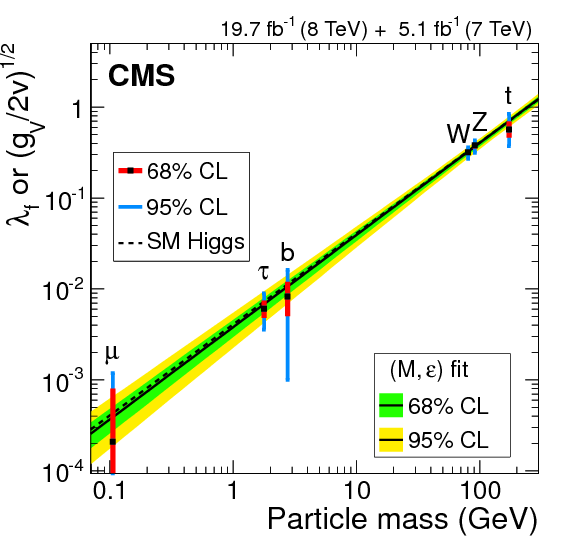
\includegraphics[width=0.80\textwidth]{coupling_ff}
    \caption{Coupling of particles to SM Higgs boson versus the mass of the particle, Log-log scale is used.}
    \label{coupling_ff}
\end{figure}



Now we should talk about the Higgs boson. First a little bit of history, an irony of life, actually. The BEH particle is called the Higgs boson, but Peter Higgs was not the first to publish the article on the BEH mechanism, he was actually the last out of BEHGHK authors! His very first article was rejected since contained no specific predictions or conclusions drawn from his calculations. This is why he was out-published by others. But this rejection made him write another article where he would explicitly state that the existence of the new boson is predicted. And this is what has made all the difference, he was the first to predict a new boson, and this boson now is called the Higgs boson. The Higgs boson is the excitation of the BEH field. Thus, the Higgs bosons can be produced at colliders by pumping more and more energy in a small space-time region exciting the BEH field "to produce" the Higgs bosons. In reality this happens making the LHC beams more energetic and thus, during the collision, having more energetic gluons (and also quarks). The main production mechanism is called a gluon fusion, when through the top quark loop a single Higgs boson is produced, this accounts for about $90\%$ of the overall LHC Higgs production at the 13 TeV energy. The second mechanism is a vector boson fusion. The third mechanism is the associated production with the weak boson. And the smallest contributor to the Higgs boson production is the ttH process, which stands for the associated production of the Higgs boson with the top anti-top quark pair (see Fig. \ref{higgs_production}). 

\begin{figure}[H]
  \centering
    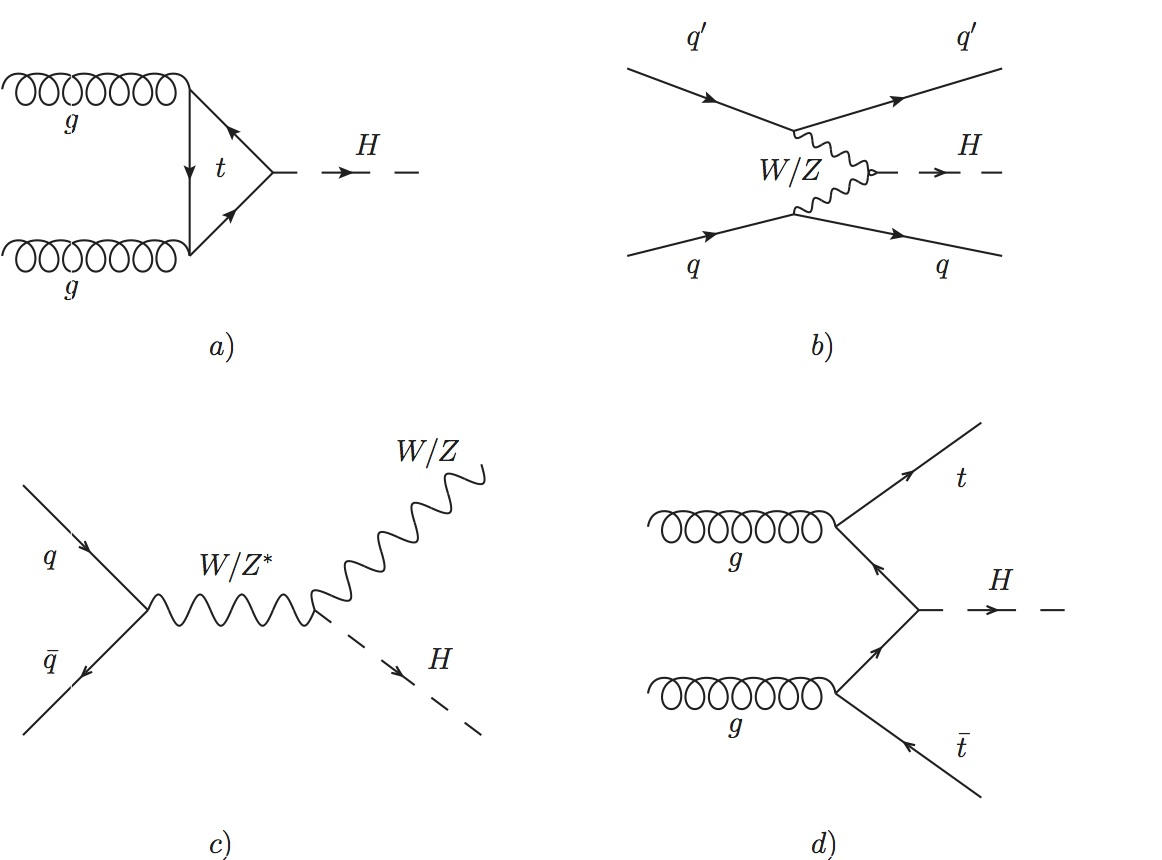
\includegraphics[width=0.90\textwidth]{higgs_production}
    \caption{SM Higgs boson production modes: a) a gluon fashion, b) a vector boson scattering,  c) an associated production with a vector boson, d) an associated production with the top anti-top pair. }
    \label{higgs_production}
\end{figure}


The final important aspect of the Higgs boson physics is the decay channels of the Higgs boson, in other words probabilities with which Higgs boson decays to other particles, so called branching fractions (see Fig. \ref{Higgs_BR_LM_RECT}). This analysis focuses on two Higgs boson decays, $H\to b\bar{b}$ and $H\to ZZ$. The first one has the highest branching ratio, while the second one gives a clean signature when subsequent $Z \to \ell\ell$ decays are selected. 




\begin{figure}[h]
  \centering
    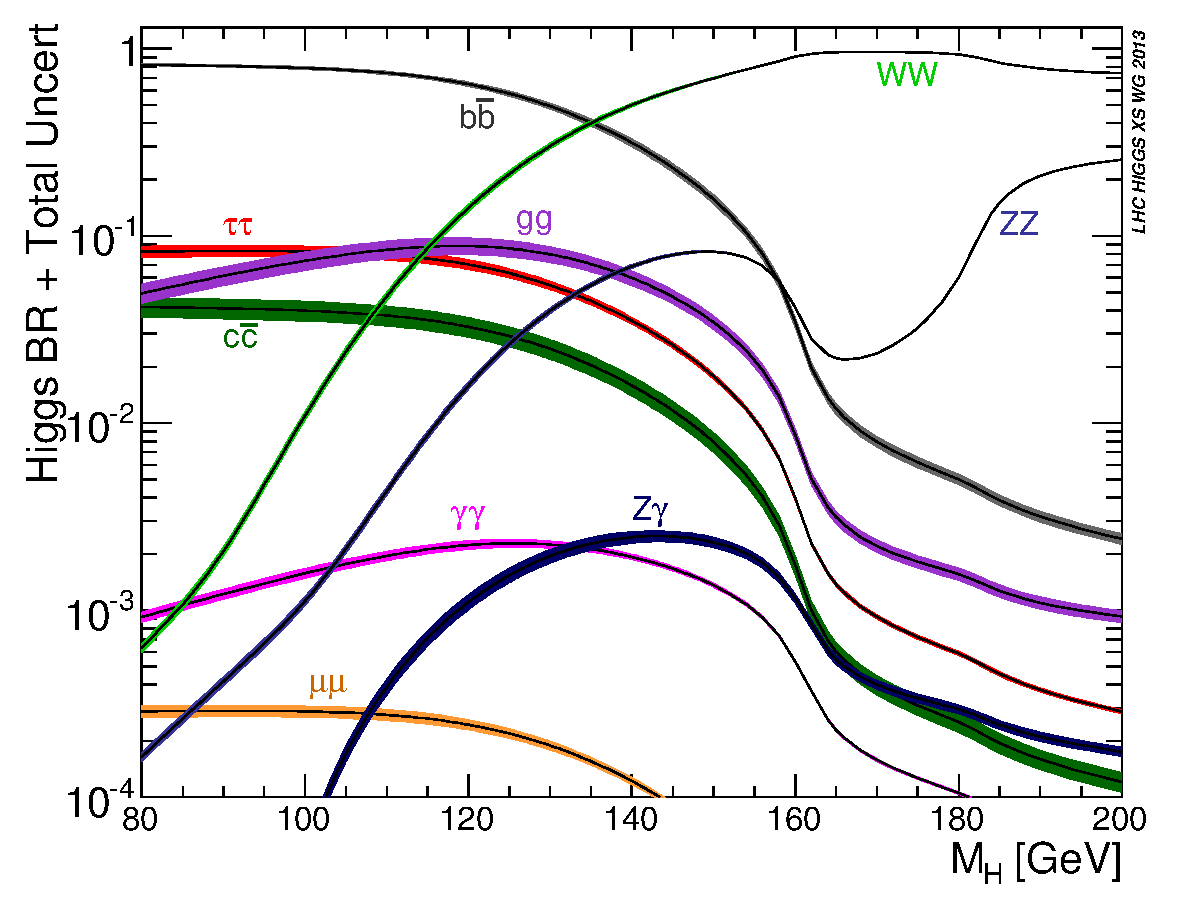
\includegraphics[width=0.90\textwidth]{Higgs_BR_LM_RECT}
    \caption{Higgs boson decay channels. At 125 GeV the dominant decay mode is $H \to b\bar{b}$.}
    \label{Higgs_BR_LM_RECT}
\end{figure}





